\chapter{Lecture 27 - Non-homogeneous Problems}
\label{ch:lec27}
\section{Objectives}
\begin{itemize}
\item Demonstrate a method for solving some non-homogeneous BVPs of the following type:
\begin{enumerate}
\item Non-homogeneous term in the PDE that is a function of no more than one independent variable; and/or
\item constant non-homogeneous term in a boundary condition.
\end{enumerate}
\item Do an example problem.
\end{itemize}
\setcounter{lstannotation}{0} %hack to try and re-set annotation counter.

\section{Time-Independent PDEs and BCs}
Consider the following BVP based on the heat equation:
\begin{table}
\begin{tabular}{l l}
$\substack{\text{Governing} \\\text{Equation}}: $& $\frac{\partial u}{\partial t} = \alpha^2 \frac{\partial^2 u}{\partial x^2} + S(x), \ \ \alpha>0, \ \ 0<x<L, \ \ t>0$ \\
& \\
$\substack{\text{Boundary} \\ \text{Conditions}}: $& $u(0,t)=u_0, \ \ u(L,t) = u_1, \ \ t>0$\\
& \\
$\substack{\text{Initial} \\ \text{Conditions}}: $ & $u(x,0) = f(x), \ \ 0<x<L $ \\
\end{tabular}
\end{table}

\noindent where $u_0$ and $u_1$ are constants.  In this boundary value problem both the governing equation and the boundary conditions are non-homogeneous.  

Since the governing equation is non-homogeneous, it is not separable.  In order to see why, let us begin the separation process:\marginnote[1.5cm]{Here we carry out the steps of separation of variables just as we did in Lecture 23.}
\begin{align*}
u(x,t) &= F(x)G(t) \\
\alpha^2 \frac{\partial^2}{\partial x^2}\left[F(x)G(t)\right] + S(x) &= \frac{\partial}{\partial t}\left[F(x)G(t)\right] \\
\alpha^2 F_{xx}G + S &= FG_t \\
\frac{\alpha^2 F_{xx}G}{\alpha^2 FG} + \frac{S}{\alpha^2 FG} &= \frac{FG_t}{\alpha^2 FG} \\
\frac{F_{xx}}{F} + \underbrace{\frac{S}{\alpha^2 FG}}_{\text{Problem!}} &= \frac{G_t}{\alpha^2 G}
\end{align*}
The term $\sfrac{S}{\alpha^2 FG}$ is a function of both $x$ and $t$ and cannot be separated.

The non-homogeneous boundary conditions are also a problem.  Suppose we were able to complete the separation process and derive separated boundary value problems for $F(x)$ and $G(t)$.  We then try to apply the spatial boundary conditions to $F(x)$:
\begin{align*}
u(0,t) &= F(0)G(t) = u_0 \\
u(L,t) &= F(L)G(t) = u_1
\end{align*}
If we had homogeneous boundary conditions and $u_0=0$---like we have always had before---we could just require $F(0)=0$ and be done with it.\sidenote{Zero is special because if $F(0)=0$, it does not matter what $G(t)$ is, we still satisfy the condition.}  But if $u_1 \ne 0$ we are stuck.  We cannot simply say: $F(0) = \sfrac{u_0}{G(t)}$; even if we knew what $G(t)$ was it could only work in the case that $\sfrac{u_0}{G(t)}$ were a constant.  The same problem applies to the boundary at $x=L$.  If we are to use separation of variables, we need to find a way to make the governing equation and boundary conditions homogeneous.

\vspace{0.25cm}

\noindent\textbf{Approach:}
\begin{enumerate}
\item Assume a solution of the form: $u(x,t) = v(x,t) + \psi(x)$.  Inserting this solution into our governing equation gives us:
\begin{align*}
\frac{\partial}{\partial t}\left[v(x,t)+\psi(x)\right]  &= \alpha^2 \frac{\partial^2}{\partial x^2}\left[v(x,t)+\psi(x)\right] + S(x) \\
v_{t} + \cancelto{0}{\psi_{t}}  &= \alpha^2 v_{xx} + \alpha^2 \psi_{xx} + S(x) 
\end{align*}

The boundary conditions become:
\begin{align*}
u(0,t) &= v(0,t) + \psi(0) = u_0 \\
u(L,t) &= v(L,t) + \psi(L) = u_1
\end{align*}
and the initial condition becomes:
\begin{equation*}
u(x,0) = v(x,0) + \psi(x) = f(x)
\end{equation*}

\item Decompose the original boundary value problem into a new, homogeneous boundary value problem for $v(x,t)$ and non-homogeneous boundary value problem for $\psi(x)$:
\begin{table}[h!]
\begin{tabular}{l l}
$\substack{\text{Governing} \\\text{Equation}}: $& $\frac{\partial v}{\partial t} = \alpha^2 \frac{\partial^2 v}{\partial x^2}, \ \ \alpha>0, \ \ 0<x<L, \ \ t>0$ \\
& \\
$\substack{\text{Boundary} \\ \text{Conditions}}: $& $v(0,t)=0, \ \ v(L,t) = 0, \ \ t>0$\\
& \\
$\substack{\text{Initial} \\ \text{Conditions}}: $ & $v(x,0) = f(x)-\psi(x), \ \ 0<x<L $ \\
\end{tabular}
\end{table}

\begin{align*}
\alpha^2 \psi_{xx} + S(x) &= 0 \\
\psi(0) = u_0, \ \ \psi(L) &= u_1
\end{align*}\marginnote[-2.0cm]{Readers are strongly encouraged to look at the boundary value problems for $v(x,t)$ and $\psi(x)$ and see that if you ``add them up'' you recover the original boundary value problem for $u(x,t)$.}
where the non-homogeneous terms from the governing equation and boundary conditions have been absorbed in the equation for $\psi(x)$.  The initial condition for $v(x,t)$ remains non-homogeneous but is modified to account for $\psi(x)$.
\end{enumerate}
We solve for $\phi(x)$, then solve for $v(x,t)$ and add the results together to get $u(x,t)$.

\vspace{0.25cm}

\noindent\textbf{Example:}  Consider the following boundary value problem:
\begin{table}
\begin{tabular}{l l}
$\substack{\text{Governing} \\\text{Equation}}: $& $\frac{\partial u}{\partial t} = \alpha^2 \frac{\partial^2 u}{\partial x^2} + S, \ \ \alpha>0, \ \ 0<x<L, \ \ t>0$ \\
& \\
$\substack{\text{Boundary} \\ \text{Conditions}}: $& $u(0,t)=0, \ \ u(L,t) = u_1, \ \ t>0$\\
& \\
$\substack{\text{Initial} \\ \text{Conditions}}: $ & $u(x,0) = f(x), \ \ 0<x<L $ \\
\end{tabular}
\end{table}

\noindent where $S$ and $u_1$ are constants, as are $\alpha^2$ and $L$; and $f(x)$ is a given function.

\vspace{0.25cm}

\noindent\textbf{Step \#1:} Substitute $u(x,t) = v(x,t) + \psi(x)$.
\begin{table}[h!]
\begin{tabular}{l l}
$\substack{\text{Governing} \\\text{Equation}}: $& $\frac{\partial v}{\partial t} = \alpha^2 \frac{\partial^2 v}{\partial x^2}, \ \ \alpha>0, \ \ 0<x<L, \ \ t>0$ \\
& \\
$\substack{\text{Boundary} \\ \text{Conditions}}: $& $v(0,t)=0, \ \ v(L,t) = 0, \ \ t>0$\\
& \\
$\substack{\text{Initial} \\ \text{Conditions}}: $ & $v(x,0) = f(x)-\psi(x), \ \ 0<x<L $ \\
\end{tabular}
\end{table}

\begin{align*}
\alpha^2 \psi_{xx} + r &= 0 \\
\psi(0) = 0, \ \ \psi(L) &= u_1
\end{align*}

\vspace{0.25cm}

\noindent\textbf{Step \#2:}  Solve for $\psi(x)$.
\begin{align*}
\alpha^2\psi_{xx}+r &= 0 \\
\psi_{xx}(x) &= -\frac{r}{\alpha^2} \\
\psi_{x}(x) &= -\frac{r}{\alpha^2}x + c_1 \\
\psi(x) &= -\frac{r}{2\alpha^2}x^2+c_1x + c_2
\end{align*}
apply boundary conditions
\begin{align*}
\psi(0) &= c_2 = 0 \\
\Rightarrow c_2 &= 0 \\
\psi(L) &= -\frac{r}{2\alpha^2}L^2 + c_1 L = u_1 \\
\Rightarrow c_1 &= \frac{1}{L}\left(u_1+\frac{rL^2}{2 \alpha^2}\right) \\
\Rightarrow \psi(x) &= -\frac{r}{2\alpha^2}x^2 + \frac{1}{L}\left(u_1+\frac{rL^2}{2 \alpha^2}\right)x
\end{align*}

\vspace{0.25cm}

\noindent\textbf{Step \#3:} Solve for $v(x,t)$.

\vspace{0.25cm}

\noindent We have already solved this problem in Lecture 23 and we will not repeat the details here.  The solution is:
\begin{align*}
v(x,t) &= \sum\limits_{n=1}^{\infty} c_n \sin{\frac{n \pi x}{L}}e^{-\left(\alpha \frac{n \pi}{L}\right)^2 t} \\
c_n &= \frac{2}{L} \int_0^L \left(f(x)-\psi(x)\right)\sin{\frac{n \pi x}{L}} \ dx
\end{align*}

\vspace{0.25cm}

\noindent\textbf{Step \#4:} Construct $u(x,t)$ from solutions for $v(x,t)$ and $\psi(x)$.

\begin{align*}
u(x,t) &= \psi(x) + v(x,t) \\
u(x,t) &= -\frac{r}{2\alpha^2}x^2 + \frac{1}{L}\left(u_1+\frac{rL^2}{2 \alpha^2}\right)x + \sum\limits_{n=1}^{\infty} c_n \sin{\frac{n \pi x}{L}}e^{-\left(\alpha \frac{n \pi}{L}\right)^2 t}
\end{align*}
\begin{marginfigure}
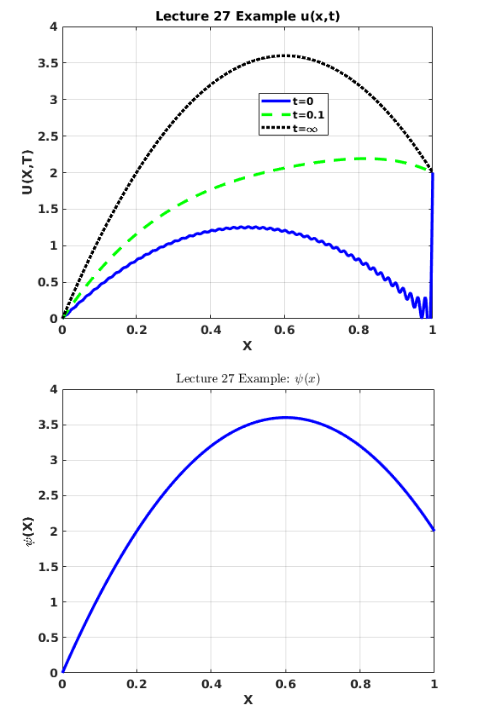
\includegraphics{lec27-ex-plt.png}
\caption{The solution, $u(x,t)$ at various times and the steady-state solution $\psi(x)$.}
\label{fig:lec27-ex-plt}
\end{marginfigure}
In this particular case, while we know from the boundary conditions, that $v(x,t)$ goes to zero as $t \rightarrow \infty$, the function $\phi(x)$ remains constant with time.  Conceptually we can think of $\phi(x)$ as being the \emph{steady state} part of the solution while $v(x,t)$ is the \emph{transient} part.

\begin{equation*}
u(x,t) = \underbrace{-\frac{r}{2\alpha^2}x^2 + \frac{1}{L}\left(u_1+\frac{rL^2}{2 \alpha^2}\right)x}_{\text{steady state}} + \underbrace{\sum\limits_{n=1}^{\infty} c_n \sin{\frac{n \pi x}{L}}e^{-\left(\alpha \frac{n \pi}{L}\right)^2 t}}_{\text{transient}}
\end{equation*}
A plot for the case: $\alpha^2 = 0.5$, $L=1$, $r=150$, $u_1=100$, and $f(x) = 300x(1-x)$ is shown in Figure \ref{fig:lec27-ex-plt}.\marginnote{
Take note of how, since the initial condition, $f(x)$, does not match the boundary condition at $x=1$ there is ``wiggliness'' in the Fourier series representation that ``diffuses away'' almost immediately.  Note also how $u(x,\infty)$ matches $\psi(x)$ as expected.} Think about the physics for a minute: we have a rod that is heated from a uniform source $r$ which gives the roughly parabolic temperature profile throughout the rod except at the ends; the left-hand side is maintained at 0 degrees and the right-hand side is held steady at 100 degrees. Hopefully the answer you see in the plot matches, more-or-less, your expectations as to what the temperature profile \emph{should} look like. 

